% !TEX encoding = UTF-8 Unicode
% !TEX root = ../../Masterthesis.tex

\chapter{Musical analysis}\label{ch:musical analysis}

\newthought{The analysis portion} of this thesis is organized into cues chronologically. Each subject cue is treated in two parts. The first part contains the primary analytical body. Following is the transcription, which ranges from a plain harmonic analysis to full-on orchestral transcriptions. The reason they are located here, and not in the end as an appendix, is because it will be handy to refer to them while reading through the analysis.

My analysis will cover several angles of approach. Mostly I will be looking at harmonic patterns, i.e. the relationship and logic between harmonic transformations, but I will comment on tonality and sonority produced by melodies and/or orchestration. Although the main body of this understanding stems from Frank Lehman's work on \acf{nRT} applied to film music, traditional analysis is very much part of the total picture. However, as I will try do describe throughout chapter \ref{ch:nrt}, the traditional way of explaining tonal progressions in relation to a traditional tonic in regard to film music is forfeit.

\begin{marginfigure}[-6cm]
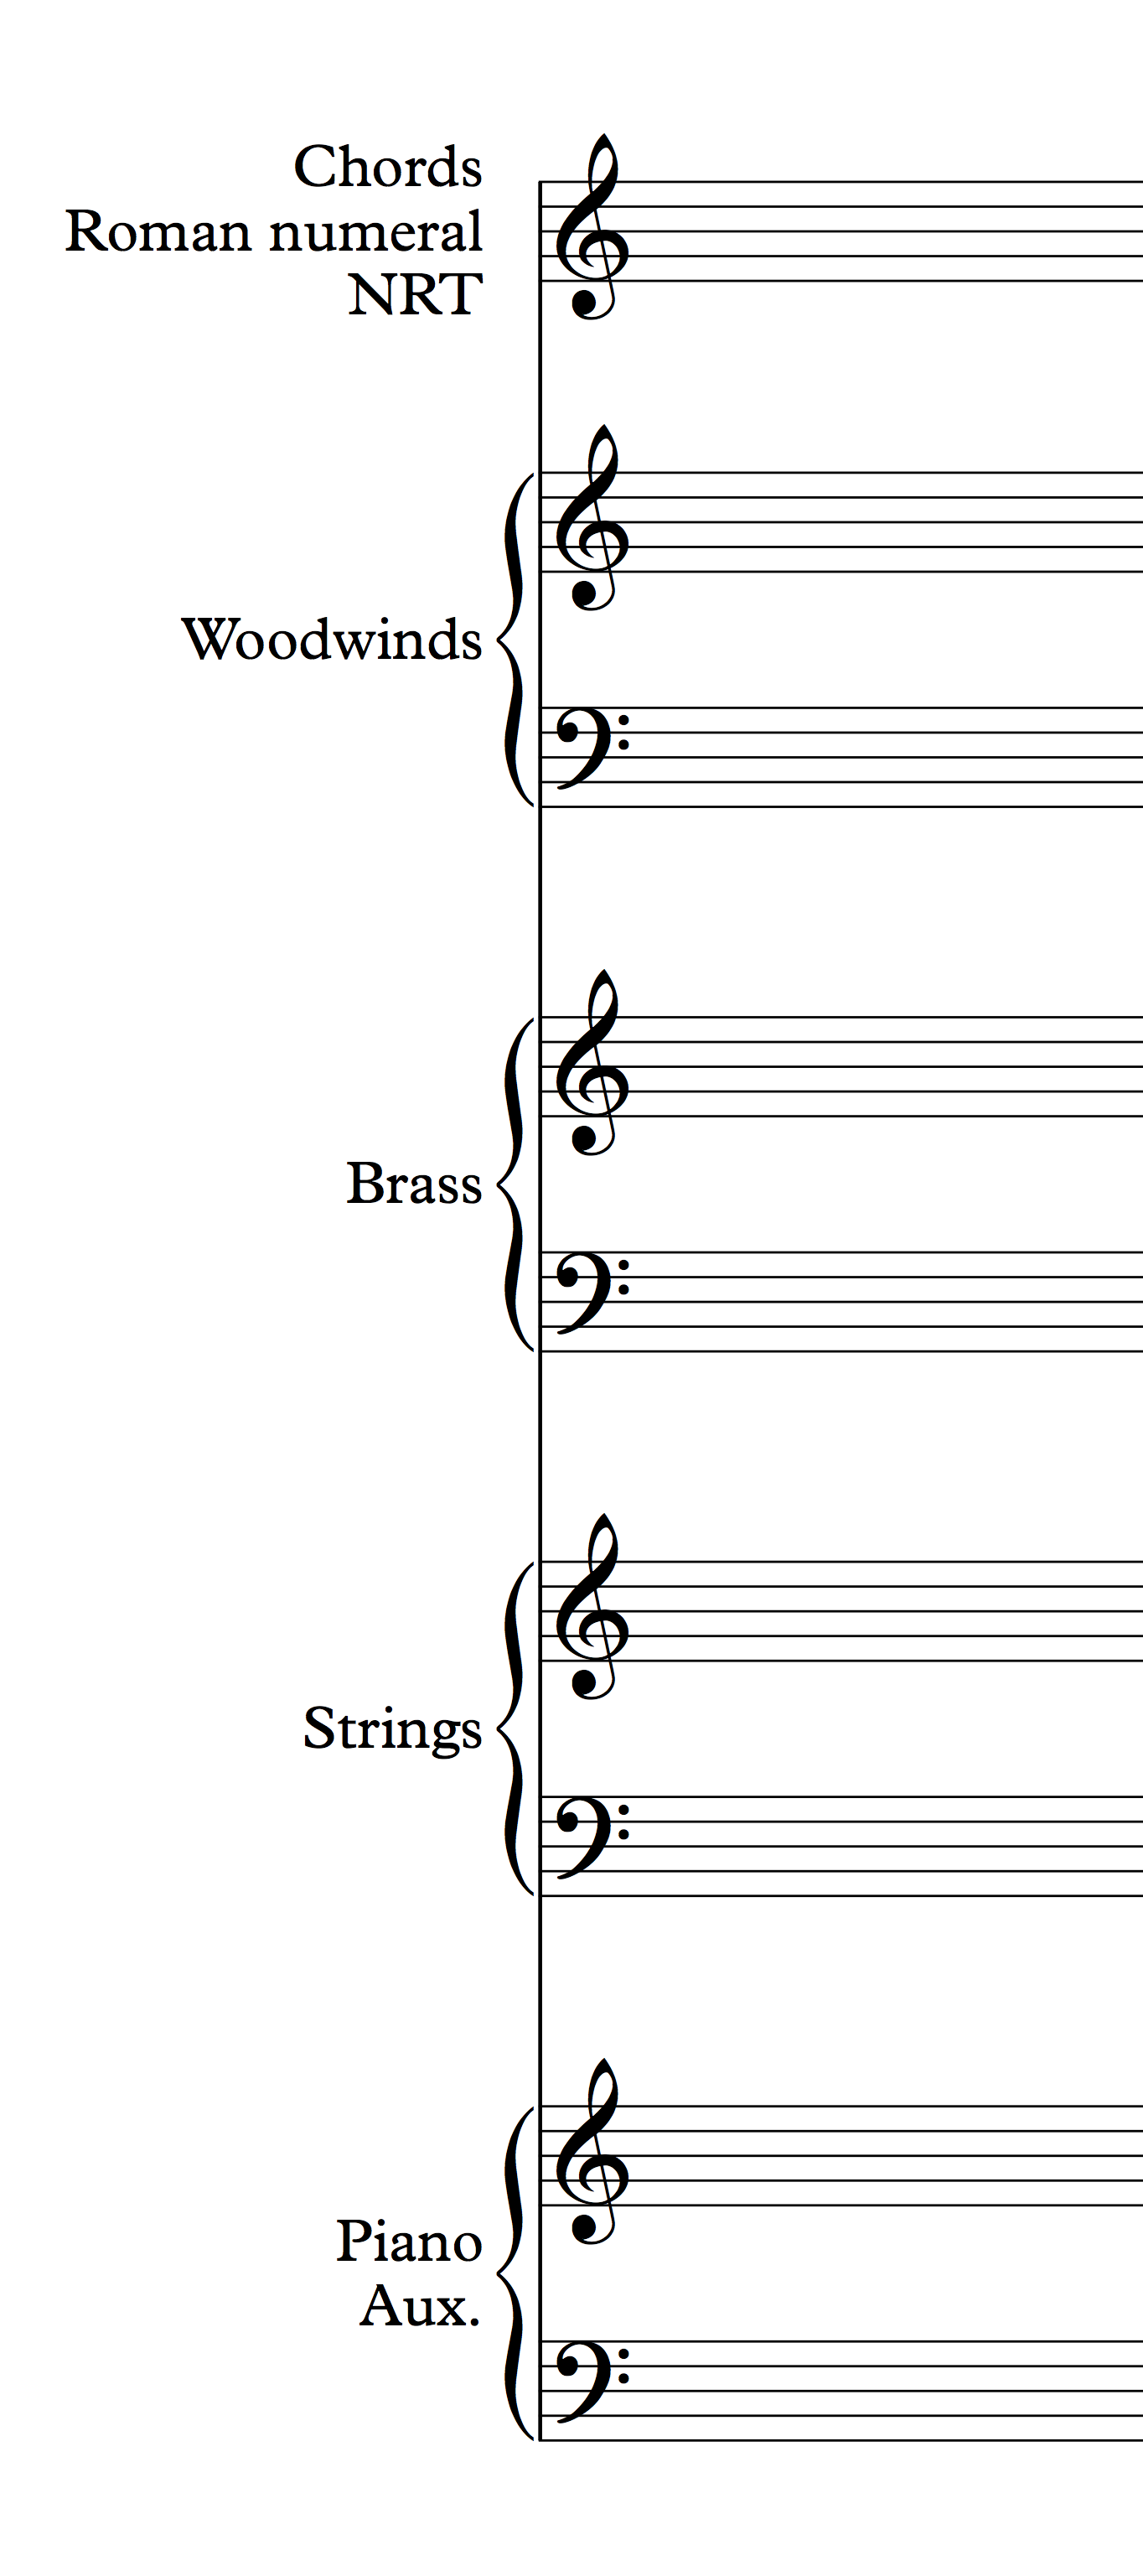
\includegraphics[width=\textwidth]{analysis_legend}
	\caption{Analysis Legend}
	\label{fg:analysis legend}
\end{marginfigure}

\begin{marginfigure}
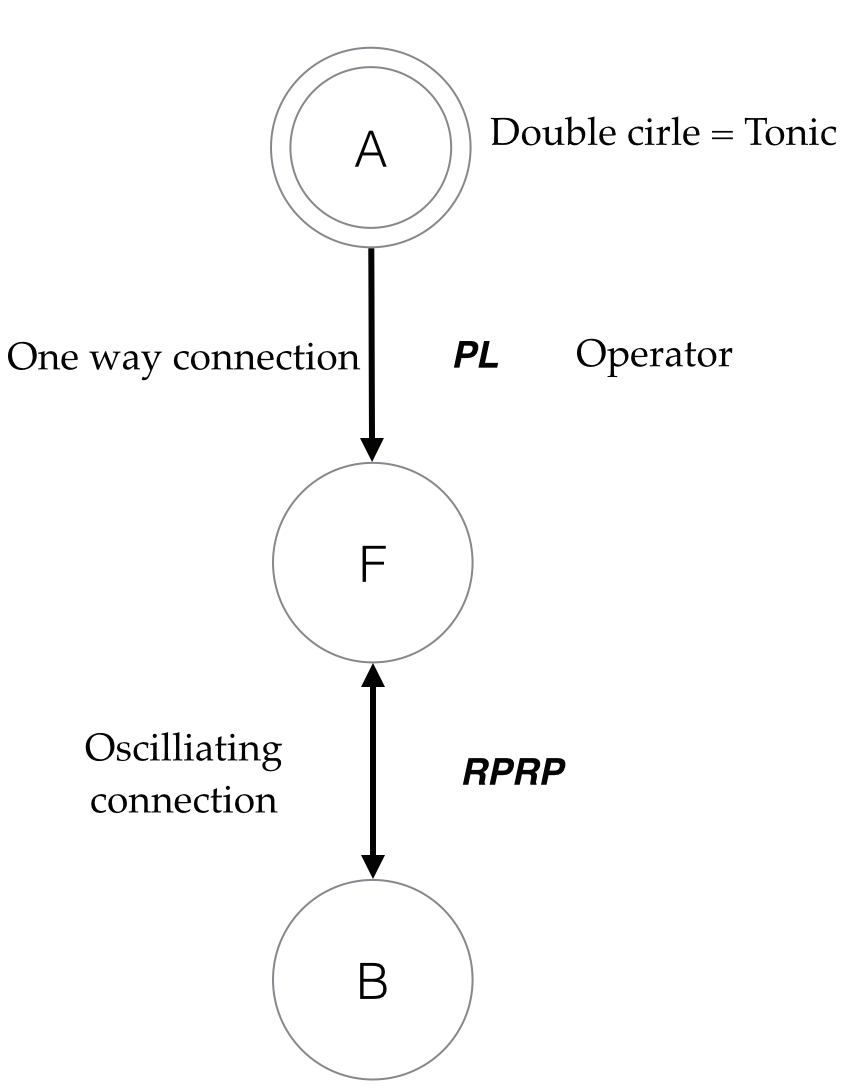
\includegraphics[width=\linewidth]{NRT_legend}
	\caption{nRT analysis legend}
	\label{fb:nrt legend}
\end{marginfigure}


In this chapter I will explain how I intend to use traditional tools. My musical background is from two very different worlds: One side of my training is classical orchestration and composition, and the other is that of a professional musician, primarily playing non-classical literature like jazz, fusion, and progressive rock. While reading academic papers on music theory, I have come across some quite creative ways to notate chords as unambiguously as possible. For the most part they feel un-intuitive for me as a musician. My solution is to alternate chord notation in two ways, both standardized in the performing world of musicians. The first and primary way is based on jazz traditions, C for C major, Cm for C minor and superscripts for added non-triadic pitches, like \chord{C}{maj7}. Superscripted integers assumes the diatonic scale except chords considered dominant, i.e. \chord{C}{7},\chord{C}{9}, \chord{C}{11} and \chord{C}{13}. Superscripted integers in parenthesis assume an alteration of that specific scale degree. The second way is to supply \textit{Schenkerian} roman numerals, using superscripts for added non-triadic pitches wherever possible or practical. I will try to use roman numerals to show scale degree but sometimes it simply is not ideal because film music is governed by what is happening on the screen, not by classical conventions. Or as Lehman puts it: \textquote[{\cite[180]{Lehman_2013}}]{It is defiantly “non-absolute” music, composed as but one part of a superordinate text.}. Thus, since film music seldom is rooted in a specific key I will refrain from giving key signatures unless very clear indications of the opposite. When practical I will draw Schenker graphs to illustrate a underlying harmonic pattern. I will indicate possible keys below the staff. \textit{Inversions} containing pitches in the root triad will be handled using the letters \(_{b, c}\) or \(_{d}\) - the latter used for hexachords and/or diminished chords. Non-triadic pitches will be displayed with a /, like C/B\(\flatx\). When sheet music is impractical, I'll refer to pitches by name or \textit{pitch classes}, (\textit{pc}), using brackets [~] and sometimes a keyboard illustration\marginnote[-2cm]{\keyboard{C,D,E,F,G,A,Bess,B}}. Unless otherwise noted, \textit{pitch class} assumes an absolute 0 regardless of key signature, making 0=C and 11=B. Step 10 and 11 are usually referred to as t and e. It is important to note that I will transpose every example given by pitch classes to C. When I need to talk about specific \textit{scale degree} in relation to a chord, I'll use a \textit{caret} to indicate this. Ex.: The \(\hat{3}\) of C=E.
